\chapter{Introduzione}
Sempre più, nella nostra realtà, sta diventando importante modellare e simulare \textit{sistemi cyber-fisici}, come droni o sistemi IoT, e \textit{sistemi biologici}, come il ciclo cellulare o ancora lo sviluppo e la propagazione di un virus. Sebbene questi due siano argomenti diversi, hanno principalmente una cosa in comune: entrambi possono essere espressi come un sistema di equazioni differenziali (o \textit{ODE}, \textit{Ordinary Differential Equation}) il quale può essere integrato sul tempo al fine di dare un "vita" al modello stesso il quale risulterà in un dataset con cui si andrà a descrivere l'andamento, in termini di valori sugli stati, quindi la \textbf{traiettoria} del sistema stesso. Questa fase di integrazione viene chiamata \textit{simulazione} del modello.

Gli \textit{eventi} sono delle situazioni alternative che deviano il normale corso della traiettoria del sistema facendole toccare punti che altrimenti non avrebbero mai considerato. Esistono quindi due tipologie di eventi: di \textit{stato} e di \textit{tempo}. I primi sorgono da condizioni sugli stati, ad esempio $x > 10$ con $x$ stato del sistema, mentre i secondi da condizioni sul tempo. Su quest'ultimi il discorso diventa più ampio però un classico evento di questo tipo scaturisce inserendo nel sistema una componente detta \textit{Sample-And-Hold}, che agisce creando una condizione sul tempo della simulazione. Una componente di \textit{Sample-And-Hold}, letteralmente "campionamento e mantenimento" è una classica componente che viene inserita all'intero di sistemi continui al fine di discretizzarne una parte di comportamento. Il nome stesso deriva dalle due azioni che questo svolge: (1) campiona il tempo della simulazione in base a dei valori che per semplicità chiameremo $start$ ed $interval$, e (2) mantiene fino al prossimo sample il valore di uno stato. Un tipico esempio è l'\textbf{Analog to Digital Converter} (ADC) il quale implementa internamente il sottosistema di s\&h\footnote{Sample-And-Hold}. Gli eventi, quindi, servono principalmente per immettere una discretizzazione all'interno di un sistema che altrimenti sarebbe continuo.\\

\begin{figure}[h]
    \centering
    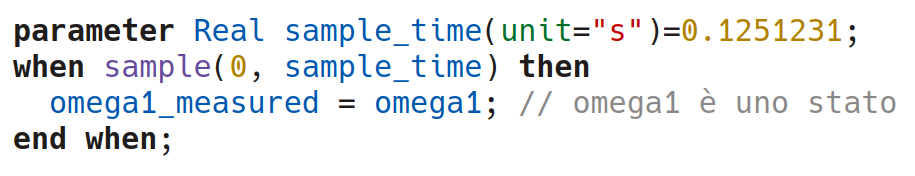
\includegraphics[width=120mm]{Intro/SH.png}
    \caption{Esempio di componente SH in Modelica.}
    \label{fig:SampleAndHoldComponentModelica}
\end{figure}
\newpage
\subsection*{Esempio1. First order system time event}
Si consideri il semplice sistema descritto da una sola equazione differenziale\footnote{Scriveremo $\dot{x}$ al posto di $\frac{\mathrm{d}}{\mathrm{d}t}x(t)$}.
\begin{equation}
    \dot{x} = (1 - x)
\end{equation}
Vediamo come questo sistema descrive semplicemente l'andamento dello stato x fino al punto 1, sul quale troverà l'equilibrio dal momento che per tutti i successivi istanti di tempo non cambierà mai di valore. Difatti il grafico della traiettoria sarà il seguente\\
\begin{figure}[h]
    \centering
    \begin{subfigure}[b]{0.4\textwidth}
        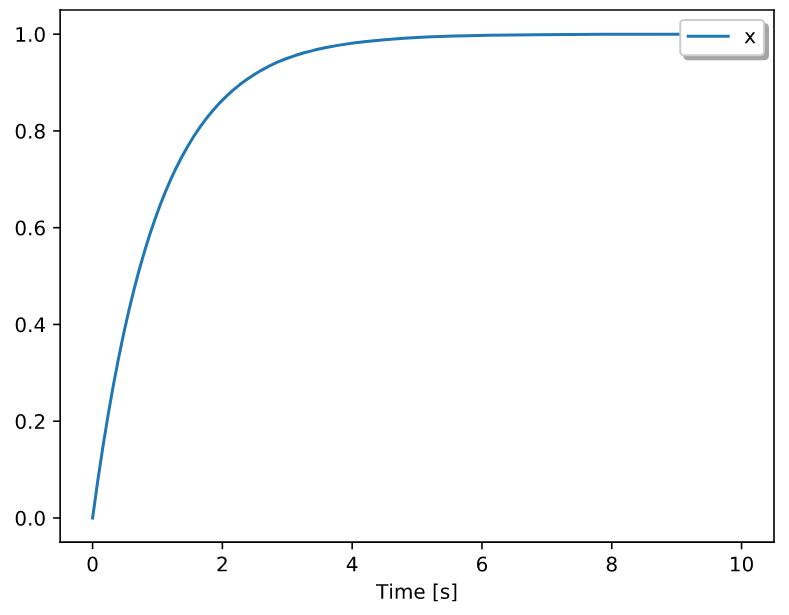
\includegraphics[width=\textwidth]{Intro/FirstOrderSystem_a.png}
        \caption{Traiettoria del sistema con valore iniziale $x=0$}
        \label{fig:my_label}
    \end{subfigure}
    \begin{subfigure}[b]{0.4\textwidth}
        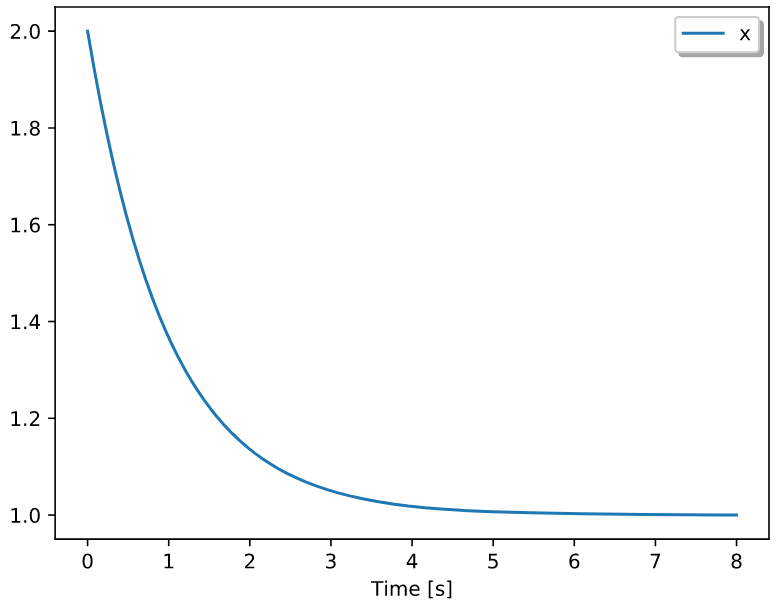
\includegraphics[width=\textwidth]{Intro/FirstOrderSystem_b.png}
        \caption{Traiettoria del sistema con valore iniziale $x=2$}
        \label{fig:my_label}
    \end{subfigure}
\end{figure}\\
Se volessimo aggiungere una componente SH all'interno del sistema per vedere il valore di $x$ a determinati istanti di tempo, decidiamo prima il tempo di sampling (es. 0.3) e implementiamo tale evento, ottenendo

\begin{figure}[!h]
    \centering
    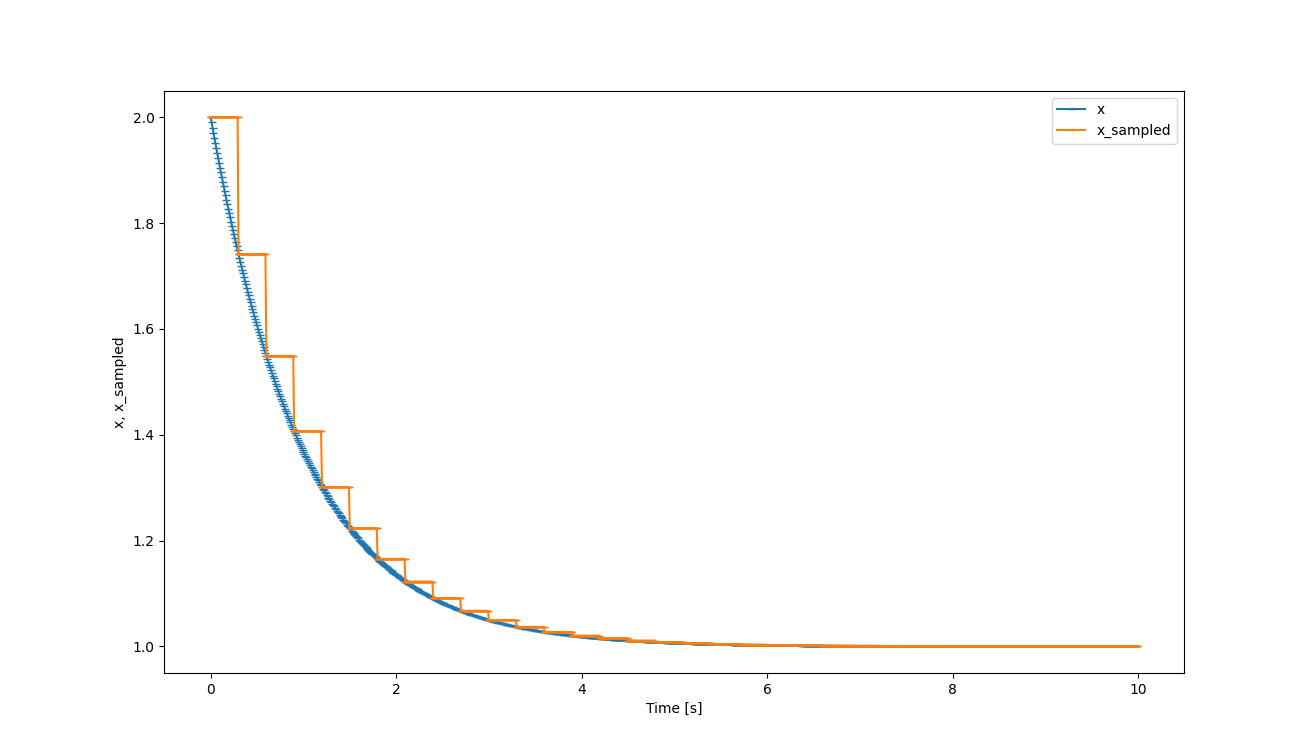
\includegraphics[width=\textwidth, height=70mm]{Intro/Plot.png}
    \caption{FirstOrderSystem con sample-and-hold e sample time di 0.3}
    \label{fig:my_label}
\end{figure}

\newpage

Questo è il codice Modelica che descrive il modello
\begin{table}[h]
    \centering
    \begin{tabular}{|p{16cm}|}
        \hline
        \begin{lstlisting}[mathescape=true, language=modelica]
model FirstOrderSystemWithSH "Semplice sistema di primo ordine"
    parameter Real x0=2.0;
    parameter Real sample_time=0.3;
    Real x;
    Real x_sampled;
initial equation
    x = x0;
    x_sampled = x0;
equation
    der(x) = (1 - x)
    when sample(0, sample_time) then
        x_sampled = x
    end when;
end FirstOrderSystemWithSH;
        \end{lstlisting}\\
        \hline
    \end{tabular}
    \label{tab:my_label}
\end{table}
\subsection*{Esempio2. FirstOrderSystem with state event}
Consideriamo adesso un secondo sistema descritto dalla seguente equazione differenziale
\begin{equation}
    \dot{x} = -\sqrt{x}
\end{equation}
Se provassimo ad eseguire una simulazione per 5 secondi, essa terminerebbe invece a 2. Questo perché le fasi di integrazioni precedenti hanno portato ad una traiettoria per lo stato x che a istanti tempi maggiori di 2 il valore potrebbe essere negativo generando quindi una \textit{floating point exception}. Per ovviare a questo problema possiamo semplicemente introdurre una condizione sullo stato x che nel momento in cui $x < 0$ allora $\dot{x} = 0$, ottenendo la seguente equazione
\begin{equation}
    \dot{x} = \begin{cases}
        -\sqrt{x}, & x \geq 0\\
        0, & altrimenti
    \end{cases}
\end{equation}